\chapter{Метод реинжиниринга встроенного программного кода}

В данной главе изложен метод реинжиниринга встроенного программного кода, рассмотрены основные типы задач, указаны особенности обработки встроенных языков. Основной акцент сделан на обработку динамически формируемого SQL-кода, однако изложенный метод может быть адаптирован к обработке систем, использующих другие встроенные языки.

\section{Особенности}

Реинжиниринг информационных систем, как правило, является комплексной задачей, которая может включать в себя различные шаги, такие как анализ кода, рефактоинг, трансформацию, перенос на другие программно-аппаратные платформы~\cite{reengANT}. При этом часто проводится всесторонний анализ многокомпонентной системы целиком, что приводит к необходимости учитывать различные особенности системы и работать с разнообразными артефактами: документацией, исходным кодом, конфигурационными скриптами, скриптами баз данных и т.д. В связи с высокой сложностью такого анализа, ренжиниринг, как правило, является автоматизированным, а не полностью автоматическим процессом, что означает возможность (и необходимость) активного участия человека.  Например, может оказаться, что в системе имеются файлы особого формата, и для их автоматической обработки потребуется создание уникального инструмента, что, в свою очередь, потребует значительных ресурсов. Однако размер этих файлов невелик и их ручной анализ прост. Таким образом, в ситуации, когда затраты на создание инструмента значительно выше затрат на ручной анализ с тем же качеством результата, часто оказывается выгоднее отказаться от создания инструмента.

При реинжиниринге информационных систем часто необходимо учитывать и динамически формируемый встроенный код. С одной стороны, такой код может содержать важную информацию о системе. Например, в динамически формируемых SQL-запросах могут содержаться сведения о схеме данных и особенностях работы с базой данных, не извлекаемые из внешнего кода. С другой стороны, при активном использовании динамически формируемый код является артефактом, требующим отдельного внимания и, следовательно, должен быть учтён, например, при оценки сложности системы, часто проводимой на начальных этапах реинжиниринга.

При большом количестве встроенного кода процесс его обработки необходимо автоматизировать. Однако, информационные системы используют встроенные языки с разной интенсивностью и разными способами. В зависимости от характера использования встроенных языков меняются требования к автоматизации их обработки: необходима ли инструментальная поддержка или ручная обработка потребует меньше ресурсов, чем создание или освоение инструмента, какими именно инструментами пользоваться в тех или иных случаях, на какие аспекты необходимо обратить внимание при принятии решений.

Необходимо отметить, что метод реинжиниринга информационных систем, учитывающий встроенный код, на настоящий момент отсутствует. Ниже такой метод представлен. Он является набором рекомендаций по выбору разработке конкретного инструментария для использования при реинжиниринге. Обработка системы сильно зависит от особенностей конкретного инструмента и решаемых задач и во многом должна быть изложена в инструкции по применению инструмента. По этой причине данный вопрос рассматриваться не будет.


\section{Метод}

Общая последовательность шагов метода представлена на рисунке~\ref{fig:method}.

\begin{figure}[ht!]
\begin{center}
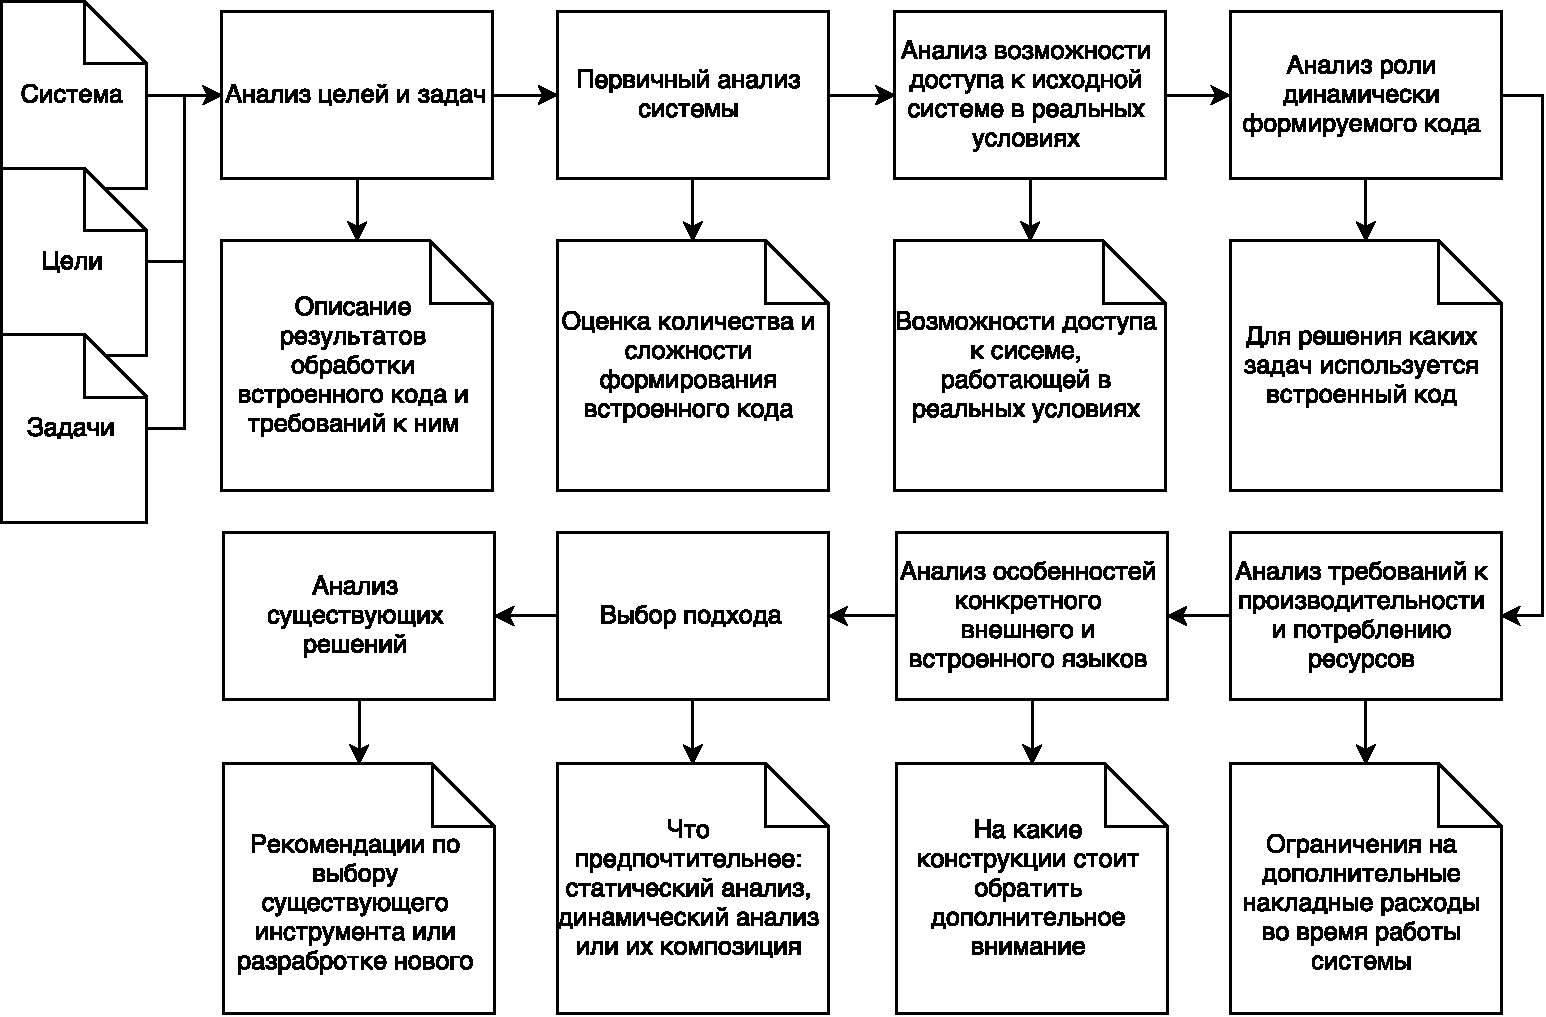
\includegraphics[width=.95\textwidth]{pics/ReengMethodSteps}
\caption{Основные шаги метода обработки встроенных языков и их результаты}
\label{fig:method} 
\end{center}
\end{figure}

В таблице~\ref{tbl:method} представлено подробное описание шагов с указанием вопросов, на которые необходимо ответить на каждом шаге и информации, необходимой для принятия соответствующих решений. Обсуждение этих шагов с описанием некоторых деталей и примеров приведено далее.

{\footnotesize
  \centering
  
  \begin{longtable}{| r | p{3cm} | p{3cm} | p{3cm} | p{6cm} |}
  
  \hline                               
  \hline
  \textnumero & Шаг & Вопросы & Ресурсы & Результат \\
  \hline 
  \endhead
  \multirow{2}{*}1 
  &
  \multirow{2}{*}{\begin{minipage}{3cm}Анализ целей и задач.\end{minipage}}
  &
  Зачем.
  &
  Цели.
  &
  Цели реинжиниринга, для достижения которых необходима обработка встроенного кода.
  \\*  
  & 
  &
  Что нужно сделать.
  & 
  Задачи.
  &
  Список задач, при решении которых необходимо обрабатывать строковые выражения.
  \\
  \hline

  \multirow{2}{*}2 
  &
  \multirow{2}{*}{\begin{minipage}{3cm}Первичный анализ системы.\end{minipage}}
  &
  Сколько в системе строковых выражений, требующих обработки.
  & 
  Исходный код системы.
  &
  Количество точек интереса в анализируемой системе. 
  \\*  
  & 
  &
  На сколько сложные строковые выражения используются.
  &
  Исходный код системы.
  &
  Количество операторов для каждой точки интереса, участвующих в формировании соответствующего запроса.
  \\
  \hline

  \multirow{3}{*}3 
  &
  \multirow{3}{*}{\begin{minipage}{3cm}Оценка доступа к исходной системе в реальных условиях.\end{minipage}}
  &
  Важность наличия доступа.
  &
  Список задач, требующих обработки строковых выражений. Результаты шага 2: наличие динамически формируемых выражений.
  &
  Есть ли задачи, решение которых упрощается при наличии доступа к работающей системе. Можно ли их решать при его отсутствии.
  \\*  
  & 
  &
  Что доступно на чтение.
  &
  Заказчик.
  &
  Какие данные и в каком объёме можно получать от работающей системы.
  \\*
  & 
  &
  Какие изменения возможно вносить в работающую систему.
  &
  Заказчик.
  &
  Какого рода изменения и в какие модули можно вносить.
  \\
  \hline
 
  \multirow{2}{*}4 
  &
  \multirow{3}{*}{\begin{minipage}{3cm}Выяснение роли встроенного кода в обрабатываемой системе.\end{minipage}}
  &
  Для чего используется встроенный код.
  &
  Код, документация, заказчик.
  &
  Функциональная и архитектурная роли встроенного кода: является ли его использование основой дизайна системы, в каких компонентах используется.
  \\*
  & 
  &
  На сколько активно используется встроенный код.
  &
  Код, документация, заказчик.
  &
  Количество точек интереса на компоненту/модуль/процедуру, на сколько интенсивно выполняется, на сколько производительность данной компоненты критична.
  \\
  \hline
 
  \multirow{4}{*}5 
  &
  \multirow{4}{*}{\begin{minipage}{3cm}Анализ производительности и вычислительных ресурсов.\end{minipage}}
  &
  Необходимо ли проводить данный анализ.
  & 
  Список задач, требующих обработки строковых выражений.
  &
  Есть ли задачи, решение которых требует дополнительных накладных расходов во время работы системы. Можно ли их решать иными способами.
  \\*  
  & 
  &
  На сколько критичен встроенный код.
  &
  Результаты шага 4.
  &
  На сколько производительность компонент, использующих встроенный код, критична для системы и на сколько она зависит от производительности встроенного кода.
  \\*
  & 
  &
  Какие существуют возможности для оценки использования и доступности вычислительных ресурсов.
  &
  Заказчик, результаты шага 3.
  &
  Есть ли возможность практически измерить потребление и доступность ресурсов.
  \\*
  & 
  &
  Есть ли запас вычислительных ресурсов.
  &
  Заказчик.
  &
  Есть ли запас вычислительных ресурсов, который можно использовать, в условиях работы целевой системы.
  \\
  \hline
 
  \multirow{2}{*}6 
  &
  \multirow{2}{*}{\begin{minipage}{3cm}Анализ языковых особенностей.\end{minipage}}
  &
  Выделение особенностей, потенциально влияющих на решение поставленных задач.
  &
  Список задач, требующих обработки строковых выражений, информация о используемых языках и средствах работы со встроенным кодом.
  &
  Список особенностей, потенциально сложных мест, обработка которых может потребовать дополнительных затрат.
  \\*
  & 
  &
  Проверка наличия выделенных особенностей в системе.
  &
  Исходный код системы.
  &
  Список особенностей, присутствующих в обрабатываемой системе, их классификация и описание.
  \\
  \hline
 
  \multirow{6}{*}7 
  &
  \multirow{6}{*}{\begin{minipage}{3cm}Выбор подхода.\end{minipage}}
  &
  Требуется ли изменение встроенного кода и сопровождение результатов.
  & 
  Цели реинжиниринга, список задач, требующих обработки строковых выражений.
  &
  На сколько естественным для разработчика должен выглядеть результат изменения встроенного кода.
  \\*  
  & 
  &
  Наличие доступа к системе, работающей в реальных условиях.
  &
  Результаты шага 3, список задач, требующих обработки строковых выражений.
  &
  Возможности по работе с системой в реальных условиях, упрощающие решение поставленных задач.
  \\*
  & 
  &
  Доступность дополнительных вычислительных ресурсов.
  &
  Результаты шага 5.
  &
  Есть ли возможность использовать дополнительные вычислительные ресурсы для динамической обработки встроенного кода.
  \\*
  & 
  &
  Требуемая точность при решении поставленных задач.
  &
  Список задач, требующих обработки строковых выражений.
  &
  Сравнение точности при решении поставленных задач с использованием динамического и статического анализа и её соотнесение с требуемой.
  \\*
  & 
  &
  Анализ особенностей.
  &
  Результаты шага 6.
  &
  Есть ли в обрабатываемой системе особенности, влияющие на выбор подхода.
  \\*
  & 
  &
  Анализ поставленных задач.
  &
  Список задач, требующих обработки строковых выражений.
  &
  Есть ли задачи, требующие строго определённого подхода к решению.
  \\
  \hline
 
  \multirow{4}{*}8 
  &
  \multirow{4}{*}{\begin{minipage}{3cm}Выбор инструмента для обработки встроенного кода.\end{minipage}}
  &
  Требуется ли структурное представление встроенного кода.
  & 
  Список задач, требующих обработки строковых выражений.
  &
  Список задач, для решения которых требуется структурное представление встроенного кода.
  \\*  
  & 
  &
  Как обрабатывать сложные случаи использования встроенного кода.
  &
  Результаты шага 6.
  &
  Дополнительные ограничения и требования, соблюдение которых необходимо для обработки сложных случаев, присутствующих в системе, и их реализуемость в рамках подходов и инструментов.
  \\*
  & 
  &
  Какой подход предпочтительнее: динамический или статический.
  &
  Результаты шага 7.
  &
  Преимущества и недостатки подходов в контексте решаемых задач и ограничений и их соотнесение с возможностями инструментов.
  \\*
  & 
  &
  Какая точность необходима при решении поставленных задач.
  &
  Цели, список задач, требующих обработки строковых выражений, заказчик.
  &
  Оценка требуемой точности при решении поставленных задач и её сравнение с возможностями подходов и инструментов.
  \\

  \hline
  \hline
  \caption{Основные шаги по подготовке к реинжинирингу системы, содержащей строковые выражения}\label{tbl:method}
  \end{longtable}
}

Рассмотрим представленные в таблице~\ref{tbl:method} шаги более подробно.

\begin{enumerate}
  \item \textbf{Анализ целей и задач реинжинирига.}
  
  На данном шаге необходимо проанализировать цели и задачи, ставящиеся в рамках проекта по реинжинирингу конкретной информационной системы. От того, какие задачи необходимо решать, напрямую зависит выбор средств и инструментов. Основные классы задач реинжиниринга информационных систем, затрагивающих динамически формируемый код, которые можно выделить на данном этапе, приведены ниже.
  
  \begin{itemize}
    \item Оценка качества кода и его сложности, что часто сводится к расчёту различных формальных метрик кода~\cite{SoftwareMetrics, DSQLQualityMesureBIG}. Здесь необходимо определить, требуется ли построение структурного представления кода для вычисления требуемых метрик с необходимой точностью.
    \item Анализ надёжности системы, поиск различного рода уязвимостей и ошибок~\cite{qualityReeng, reengErrors}. При этом требуется изучение типов ошибок, которые предполагается обнаруживать: обнаружение некоторых типов ошибок требуют построения структурного представления кода (семантические ошибки), в то время, как в других случаях это не требуется (лексические, синтаксические ошибки).
    \item Извлечение или восстановлении утраченных знаний о системе~\cite{reengANT, qualityReeng}. В зависимости от деталей этой задачи может потребоваться динамический анализ или структурное представление встроенного кода.
    \item Трансформация исходной системы: рефакторинг, перенос на новые программно-аппаратные системы~\cite{reengANT, qualityReeng}. Для решения подобных задач, как правило, требуется структурное представление кода.
  \end{itemize}
  
Особенно важен данный шаг при необходимости решать задачи трансформации динамически формируемого кода. Например, если необходимо как можно быстрее получить работающую систему, дальнейшее развитие которой не планируется, то можно пожертвовать качеством кода результирующей системы, что может существенно упростить его обработку. Однако, если после выполнения трансформации планируется активная разработка или поддержка полученной системы, то к результирующему коду предъявляются дополнительные требования. Важными становятся, например, форматирование кода, его однородность (использование нескольких диалектов SQL вместо одного затрудняет работу с кодом), требуется сохранить не только внешнее поведение системы, но и её внутреннюю структуру на всех уровнях (пакеты, модули, процедуры). Выполнение этих условий упростит дальнейшую работу с кодом системы, позволит уменьшить затраты на обучение команды, поиск новых специалистов.
  
  Например, при трансляции с одного диалекта на другой хранимого SQL-кода который активно использует динамический SQL, важно сохранить однородность результирующей системы в том смысле, что и основной код и встроенный должны быть быть написаны на одном и том же диалекте. Это особенно важно, если планируется дальнейшее развитие системы. Обусловлено это тем, что различные диалекты SQL содержат большое количество особенностей и разработчики на SQL часто оказываются специалистами достаточно узкого профиля. Таким образом, наличие двух различных диалектов вместо одного может усложнить набор команды. Более того, в процессе разработки необходимость переключаться между несколькими диалектами так же может вызвать трудности.
  
  Таким образом, один из основных вопросов, на которые необходимо ответить при анализе целей: планируется ли активное изменение системы после её реинжиниринга, если он включает трансформации.
  
  \item \textbf{Первичный анализ проекта.} На данном этапе необходимо проанализировать исходный код информационной системы и выяснить характеристики встроенного кода. Для этого, как правило, можно использовать стандартные средства статического анализа программного кода. Однако, скорее всего, они будут требовать модификации, поэтому необходимо иметь доступ к исходному коду этих инструментов. Необходимо оценить следующие характеристики кода информационной системы.
  \begin{itemize}
    \item Количество точек интереса --- тех точек, где сформированное строковое выражение передаётся на обработку соответствующей компоненте. Это позволит оценить интенсивность использования встроенного кода. Как правило, за выполнение выражений на встроенном языке отвечают характерные языковые конструкции, например \verb|EXECUTE| в языке T-SQL. следовательно, необходимо оценить количество таких конструкций. Для грубой оценки можно использовать простой текстовый поиск. Он может оказаться полезным, так как если такой поиск говорит о полном отсутствии соответствующих конструкций, то дальнейший анализ можно не проводить. Для более точной оценки необходимо использовать структурное представление кода, чтобы, например, не учитывать код, находящийся в комментариях. Получить структурное представление и доступ к нему можно с помощью библиотек синтаксического анализа соответствующего языка.
    
    \item Сложность формирования строковых выражений. Прежде всего необходимо определить наличие динамически формируемого кода и оценить сложность его формирования, так как в случае использования только константных строковых литералов не потребуется специальных инструментов для анализа встроенного кода.
    
    Для данной оценки можно использовать алгоритм протягивания констант~\cite{Dragon}, являющееся одним из стандартных шагов при статическом анализе кода. Однако потребуется его модификаций. Необходимо, чтобы отдельно обрабатывались выражения, отвечающие за формирование кода, и собиралась следующая информация о процессе формирования кода как для каждой точки выполнения, так и для всей системы в целом.
    \begin{itemize}
      \item Количество конкатенаций.
      \item Количество операторов ветвления: \verb|if-then-else|, \verb|switсh-case| и т.д.
      \item Количество строковых функций: \verb|replace|, \verb|substring| и т.д.
      \item Количество циклов, как ``явных'' (\verb|while|, \verb|for|), так и организованных с помощью рекурсии.
      \item Количество переменных, значение которых нельзя полностью вычислить статически (например, они получают значение из пользовательского ввода).
      \item Факт формирования кода в ``телах'' более чем одного метода/процедуры. Для получения данной информации в используемом инструменте необходима поддержка межпроцедурного анализа.
    \end{itemize}
  \end{itemize}

  \item \textbf{Возможности доступа к исходной системе в реальных условиях.} Возможность изучения системы в реальных условиях может дать большое количество полезной информации, например интенсивность выполнения встроенного кода, что трудно или даже невозможно получить другими способами, так как даже тесты часто не воспроизводят реальные сценарии функционирования системы. Однако такой доступ часто оказывается невозможным или крайне затруднённым, что вызывается, с одной стороны, вопросами безопасности, с другой стороны, отсутствием возможности гарантировать, что внесение изменений, необходимых для получения требуемой информации (например, ведение дополнительного журнала) не отразятся на работоспособности системы.  
  \begin{itemize}
    \item Необходимо определить, есть ли доступ к системе, работающей в реальных условиях и что именно доступно: чтение определённых журнальных файлов, перехват сообщений на каком-либо уровне, доступ к базе данных системы.
    \item Необходимо выяснить, модификации какого рода разрешены, какая информация не является закрытой и может быть передана разработчикам. Это влияет на то, какие задачи можно решать при помощи динамического анализа.
    \item Необходимо определить, возможен ли запуск модифицированной системы в реальных условиях. Если это возможно, то важно убедиться, что будет возможность получить доступ к собранной информации. Наличие такой возможность может позволить, например, собрать информацию о том, с какими объектами работают с использованием динамически формируемых запросов при выполнении конкретных сценариев.
  \end{itemize}

  
  \item \textbf{Роль динамически формируемого кода в системе.} На данном шаге необходимо определить, какую роль в системе играют динамически формируемые запросы. Возможны следующие существенно различные ситуации.
  \begin{itemize}
    \item Использование динамически формируемого кода является один из основных элементов архитектуры системы. Данная ситуация, как правило, характеризуется большим количеством точек исполнения и наличием сложно формируемого кода. Важно определить, какие именно компоненты системы построены таким образом, так как использование встроенных языков может быть неоднородным. Средние значения по всей системе могут быть не велики, при этом ряд ключевых компонент могут быть построены с активным использованием динамически формируемого кода, а в остальных он отсутствует. При этом может оказаться, что ключевые компоненты являются ещё и самыми критическими по производительности частями системы.
    
    \item Динамически формируемый код используется как вспомогательное средство. Явным признаком такой ситуации является малое количество или полное отсутствие такого кода, но это не всегда так. Возможна ситуация, когда динамически формируемых код активно используется для реализации служебной и вспомогательной функциональности, например, для сбора статистики, администрирования и диагностики системы. Тот факт, что данная функциональность не является основной для системы, может позволить обращать меньше внимания, например, на производительность результатов трансформации встроенного кода. Это даёт больше возможностей для использования динамического подхода, так как накладные расходы на дополнительные вычисления во время работы системы не окажут существенного воздействия на производительность основных её функций.
  \end{itemize}
    
  \item \textbf{Анализ требований к производительности и потреблению ресурсов.} Необходимо определить, позволительны ли дополнительные накладные расходы на обработку встроенного кода при работе реальной системы. Ответ на данный вопрос особенно важен, например, при выборе между статическим и динамическим подходом к трансляции динамически формируемого кода. Выполнение динамически формируемых SQL-запросов само по себе требует дополнительных ресурсов. Если на предыдущих шагах было выяснено, что динамически формируемый код активно используется в критическом по производительности фрагменте системы, а вычислительные ресурсы ограничены, то применение динамического подхода неприемлемо. Это связано с тем, что дополнительные вычисления для обработки кода существенно ухудшат быстродействие критических фрагментов системы.
  
  \item \textbf{Анализ особенностей конкретного внешнего и встроенного языков.} Многие задачи требуют комплексной обработки внешнего и встроенного кода. Например, при статическом поиске ошибок, включающем ошибки использования типов переменных, необходимо проводить анализ, проверяющий, что тип переменной во внешнем коде соответствует типу, возвращаемому запросом. Пример несовпадения типов приведён в листинге~\ref{lst:typeChecking}: переменная \texttt{result} имеет тип \texttt{List<string>}, однако запрос возвращает коллекцию двухэлементных кортежей.
  
\fvset{frame=lines,framesep=5pt}
\begin{listing}
    \begin{pyglist}[language=csharp,numbers=left,numbersep=5pt]

public List<string> NewReport
  (int prodId = 0, int status = 0, int nType = 0)
{
    int nProdIdL = prodId;

    string sMagicKey = "[" + prodId.ToString() + "]";

    string tbl = status == 0 ? "InOrders " : "OutOrders ";

    while (nProdIdL > 0)
    {
        sMagicKey = "[" + sMagicKey + "]";
        nProdIdL = nProdIdL - 1;
    }

    string sExec =
        "SELECT sOrderDescription, " + sMagicKey
        + " FROM ts." + tbl;

    List<string> result = db.Execute(sExec);
    return result;
}
\end{pyglist}
\caption{Пример кода метода на языке программирования C\#, в котором ожидаемый и реальный тип результата запроса не совпадают}
\label{lst:typeChecking}
\end{listing}

  Наличие некоторых связей внешнего и встроенного кода делает невозможным полностью динамический подход, так как без статического анализа не будет получена информация, необходимая для корректного преобразования внешнего кода. Примером такой ситуации может служить трансформация кода хранимой процедуры с динамическими запросами, формирующими запрос \verb|SELECT| из T-SQL в PL-SQL. При этом результат данного запроса должен быть результатом процедуры. В T-SQL вне зависимости от типа сформированного запроса его выполнение производится с помощью команды \verb|EXECUTE| и результат выполнения автоматически возвращается в качестве результата процедуры, а в PL-SQL для того, чтобы получить результат выполнения запроса и вернуть его наружу из процедуры необходимо использовать конструкцию \verb|EXECUTE IMMEDIATE ... INTO out_var|~\footnote{Языковая конструкция, которая позволяетвыполнить запрос и сохранить результат его выполнения в переменной~\cite{PLExecute}.}, при этом \verb|out_var| должна быть объявлена аргументом процедуры с модификатором \verb|OUT|~\footnote{Модификатор \texttt{OUT} для аргумента подпрограммы означает его передачу по ссылке, что позволяет возвращать его значение в вызывающую подпрограмму~\cite{PLProc}.}. То есть в данном случае без статического анализа динамически формируемого кода невозможно корректно преобразовать внешний код.

  Отдельно нужно проверить наличие конструкций, которые заведомо усложняют автоматическую обработку системы. Примером такой конструкции может служить оператор \verb|MERGE|\footnote{Операция позволяющая одновременно добавлять новые записи и обновлять существующие~\cite{PLMerge}.} в PL-SQL, проекция которого в другие языки может потребовать существенных усилий.
  
  \item \textbf{Выбор подхода.} Основной вопрос, который необходимо решить на данном шаге --- это выбор между статическим и динамическим подходом или их композицией. На предыдущих шагах могли быть выявлены особенности, накладывающие ограничения на выбор. Может оказаться, что необходим не чистый статический~\cite{Syrcose} или динамический~\cite{DynamicDSQLTranslation} подходы, а их смесь. Такая ситуация возникает, например, когда решение задачи с помощью статического анализа крайне затруднено или невозможно, но динамический подход требует неприемлемых накладных расходов. В данном случае может быть применён смешанный подход. Примером может послужить обработка конструкции \verb|MERGE|, статическая проекция которой сложна. В данном случае на этапе статического анализа вычисляется вся информация, необходимая для трансформаций во время выполнения, которая может быть вычислена, и сохраняется, например, в специальных переменных. Далее, во время выполнения происходит окончательная трансформация кода и наличие заранее вычисленной информации сокращает накладные расходы.
  
  \item \textbf{Выбор инструмента для обработки встроенного кода.} Результатом проделанного анализа должно стать решение о том, какими именно средствами проводить анализ встроенного кода. С одной стороны, необходимо выбрать готовый инструмент, если это возможно. Обзор основных существующих решений  приведён в разделе~\ref{SELToolsDescr} данной работы. Рассмотрим ситуаций, в которых возможно использование рассмотренных инструментов.
  \begin{itemize}
    \item Статический поиск синтаксических ошибок может быть автоматически проведён с помощью таких инструментов как JSA~\cite{JSAUrl} или PHPSA~\cite{PHPSAUrl} для сложно формируемых выражений. Для детальной диагностики может потребоваться применение таких инструментов, как Alvor~\cite{AlvorUrl}, IntelliLang~\cite{IntelliLang} или PHPStorm~\cite{PHPStorm}.
    \item Статическая трансформация встроенного кода, каждое выражение которого полностью содержится в константном литерале, может быть автоматически осуществлена SQL Ways~\cite{SQLWays}.
    \item Для интерактивного изучения кода на PHP со встроенным HTML и JavaScript может использоваться Varis~\cite{Varis}.
    \item Статическая трансформация встроенного кода со сложной логикой формирования может быть автоматизирована с помощью инструментов, разработанных на основе платформы, аналогичной представленной в данной работе.
  \end{itemize}
  
  С другой стороны необходимо определить границы автоматизации процесса, то есть определить, какая часть работ выполняется с помощью инструментов (автоматически), а какая --- вручную. Провести чёткое разделение крайне сложно, так как возможны различные ситуации в диапазоне от наличия готового инструмента, решающего необходимые задачи и специалистов, умеющих с ним работать, до отсутствия инструмента и специалистов, способных его создать. В такой ситуации характеристики системы, оцененные на предыдущих шагах, не являются решающим фактором в принятии решения о ручной обработке или автоматизации и её границах, однако являются необходимым условием для принятия правильного решения.
  
  Кроме того, после изучения существующих инструментов, может быть  принято решение о необходимости разработки собственного. В таком случае, проведённый анализ позволит сформулировать требования к нему, а основой для разработки может стать инструментальный пакет, предложенный в данной работе.
  
\end{enumerate}

Использование изложенного выше метода позволяет принять решение о способе и инструментах обработки встроенного кода в системах, использующих встроенные языки, в контексте реинжиниринга. При этом метод учитывает такие характеристики динамически формируемого кода, как частота использования, сложность формирования выражений, его роль в системе, особенности целей и задач обработки системы.


\clearpage
